%!TEX root = Manuscript.tex

\chapter{Precise matching}
\label{chap:intro}
\minitoc

\section{Introduction}
\subsection{Motivation}
\subsection{Contribution}
check SIFT scale and rotation\\
\textit{one-to-one tiling scheme}\\
3D ransac?

\section{Methodology}
To compute precise {inter-epoch} matches, we perform matching on original RGB images {under the guidance of co-registered orientations and DSMs}. {It consists of extracting tentative inter-epoch matches, followed by a 3D-RANSAC filter and a cross correlation stage to remove outliers.} The workflow is displayed in Figure~\ref{WorkflowPatch}(a).
\par
We choose matching RGB images for precise matching instead of DSMs, as the DSMs are noisy due to low radiometric quality of the images. In Appendix~\ref{chap:appendix4} we compared the matching results on RGB images and DSMs over the same area. It demonstrated that there are more numerous but less accurate matches found in DSMs. As the goal of precise matching is to recover accurate matches, the RGB images are more suitable than DSMs.\\

\begin{figure*}[htbp]
	\begin{center}
		\subfigure[Workflow]{
			\begin{minipage}[t]{1\linewidth}
				\centering
				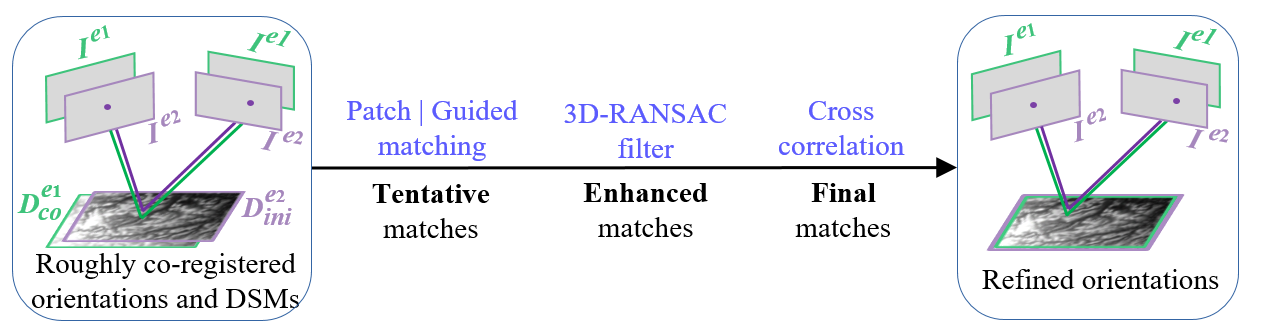
\includegraphics[width=1\columnwidth]{images/Chapitre4/precisematching.png}
			\end{minipage}%
		}
		\subfigure[Patch matching]{
			\begin{minipage}[t]{0.35\linewidth}
				\centering
				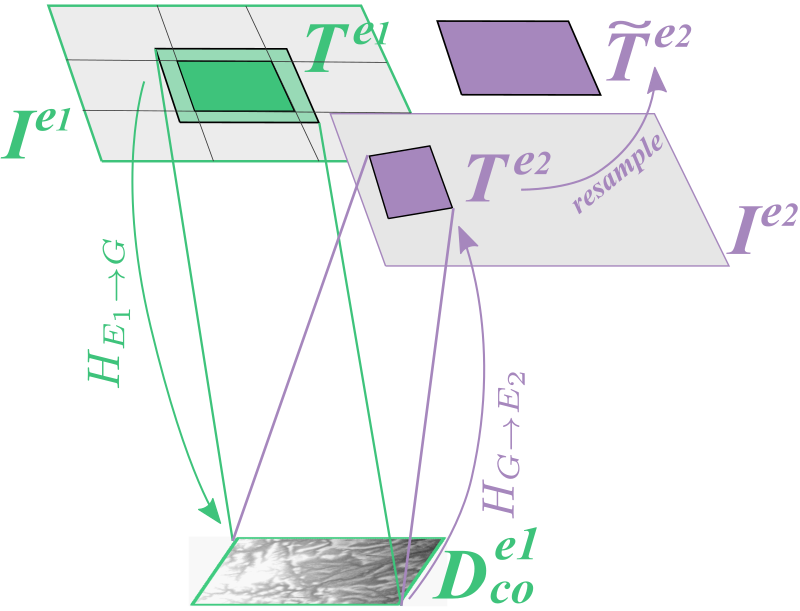
\includegraphics[width=4.5cm]{images/Chapitre4/patchmatching.png}
			\end{minipage}%
		}
		\subfigure[Buffer zone of tiles]{
			\begin{minipage}[t]{0.25\linewidth}
				\centering
				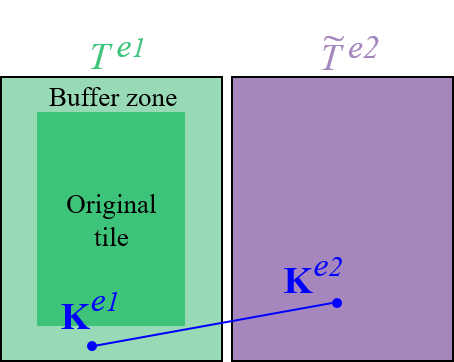
\includegraphics[width=3.8cm]{images/Chapitre4/tilingScheme.png}
			\end{minipage}%
		}
		\subfigure[Guided matching]{
			\begin{minipage}[t]{0.35\linewidth}
				\centering
				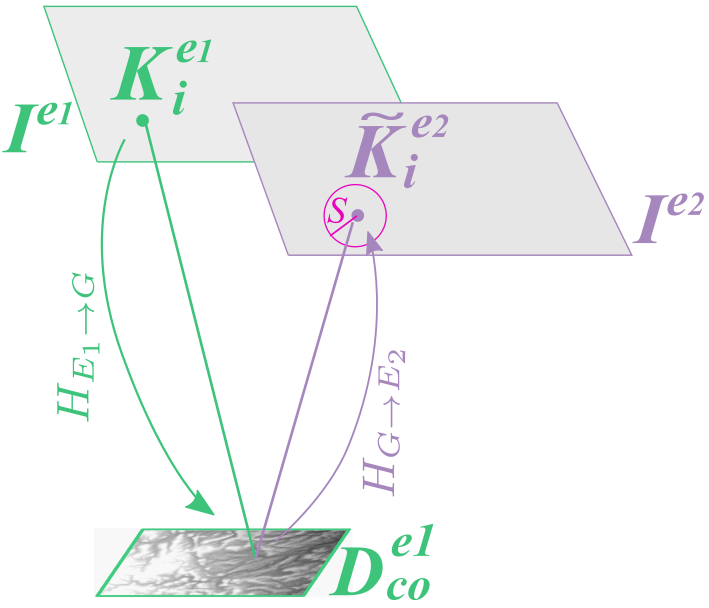
\includegraphics[width=4.5cm]{images/Chapitre4/guidedmatching.png}
			\end{minipage}%
		}
		\caption{(a) Workflow of precise matching. It is carried out by performing patch or guided matching to obtain tentative matches, followed by 3D-RANSAC filter and cross correlation, giving rise to final matches. (b) and (d) illustrate toy-examples of the patch matching and guided matching, respectively. (c) displays the feature correspondences where $\mathbf{K}^{e_1}$ exceeds the original tile size (dark green area) and therefore will be abandoned.}
		\label{WorkflowPatch}
	\end{center}
\end{figure*}

\subsection{Get tentative matches}\label{patch matching}
We offer two alternatives to recover tentative matches: patch or guided matching. {The former has better overall} performance while the latter is more efficient in terms of the use of memory and CPU resources.\\
\subsubsection{Patch matching for learned features}
{{It} is based on \textit{one-to-one tiling scheme}} {(not to confuse with the \textit{one-to-many tiling scheme} presented in the \textit{rough co-registration}), as shown in Figure~\ref{WorkflowPatch}(b) and detailed below}:
\begin{enumerate}
	%\item Crop the master RGB image $I^{e_1}$ into M tiles ($T^{e_1}$) of certain size (640$\times$480 pixels in our experiments), with a buffer zone (64 pixels in the width and 48 pixels in the height in our experiments) overlapped with each other;
	\item Crop the master RGB image $I^{e_1}$ into M original tiles of certain size, and expand them with a buffer zone (as shown in Figure~\ref{WorkflowPatch}(c)), giving rise to M buffered tiles ($T^{e_1}$);
	\item Project each buffered tile $T^{e_1}$ onto the DSM $D_{co}^{e_1}$ and backproject to secondary RGB image $I^{e_2}$ to find the corresponding tile $T^{e_2}$;
	\item Resample $T^{e_2}$ to $\widetilde{T}^{e_2}$, so that the tile pair $P({T^{e_1},\widetilde{T}^{e_2}})$ is free from differences of rotation, scale and extent;
	\item Apply SuperGlue on tile pair $P({T^{e_1},\widetilde{T}^{e_2}})$ to find matches $M({\mathbf{K}^{e_1},\mathbf{K}^{e_2}})$ ($\mathbf{K}^{e_i}$ represents keypoints in $I^{e_i}$);
	\item Merge together the matches from M tile pairs by removing the matches with $\mathbf{K}^{e_i}$ located in the buffer zone.\\
\end{enumerate}

Because the orientations and DSMs are only roughly co-registered, we have to take into account the margin of error when projecting tiles to overlapping images. This is why we add a buffer zone in the tile $T^{e_1}$. In our experiments, the sizes of original and buffered tiles are set to 512$\times$384 and 640$\times$480 pixels individually.\\
For better understanding, in Figure~\ref{patchexample} we displayed an example of an inter-epoch image pair, as well as the tile pairs resulted from the \textit{one-to-one tiling scheme}.\\
Our patch matching experiments are performed based on SuperGlue, however, other learned methods can be adopted readily. \\

\begin{figure*}[htbp]
	\begin{center}
		\subfigure[Example of an image pair]{
			\begin{minipage}[t]{1\linewidth}
				\centering
				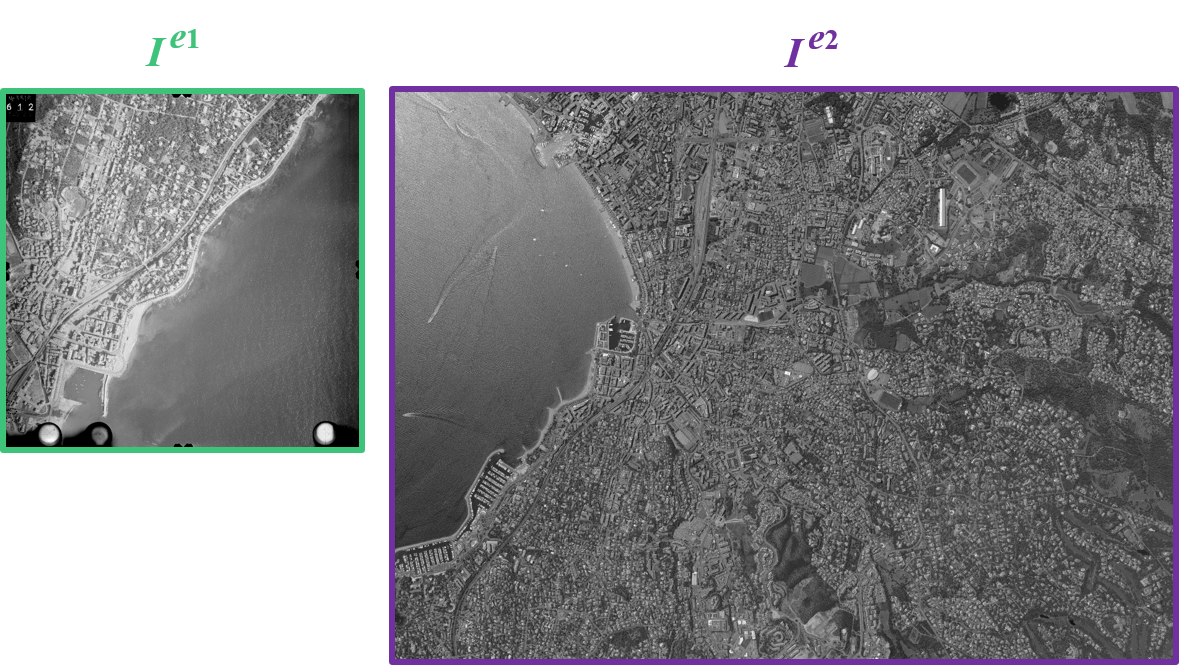
\includegraphics[width=1\columnwidth]{images/Chapitre4/example.png}
			\end{minipage}%
		}
		\subfigure[Example of patch pairs]{
			\begin{minipage}[t]{1\linewidth}
				\centering
				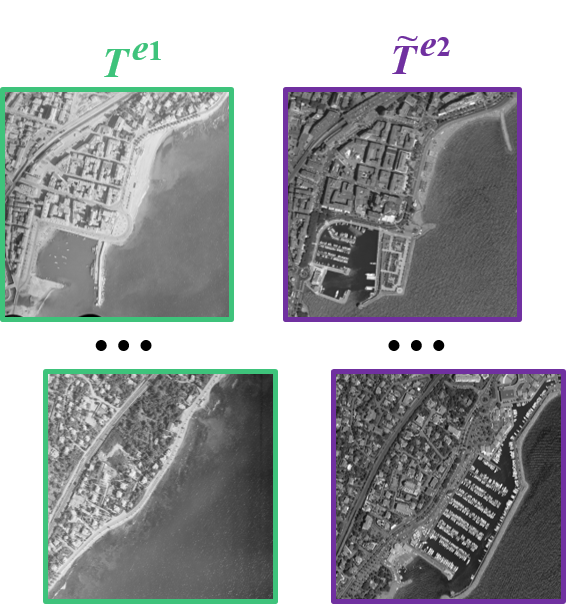
\includegraphics[width=1\columnwidth,trim=10 0 0 0,clip]{images/Chapitre4/patchexample.png}
			\end{minipage}%
		}
		%			\subfigure[Example of keypoint prediction]{
		%		\begin{minipage}[t]{1\linewidth}
		%			\centering
		%			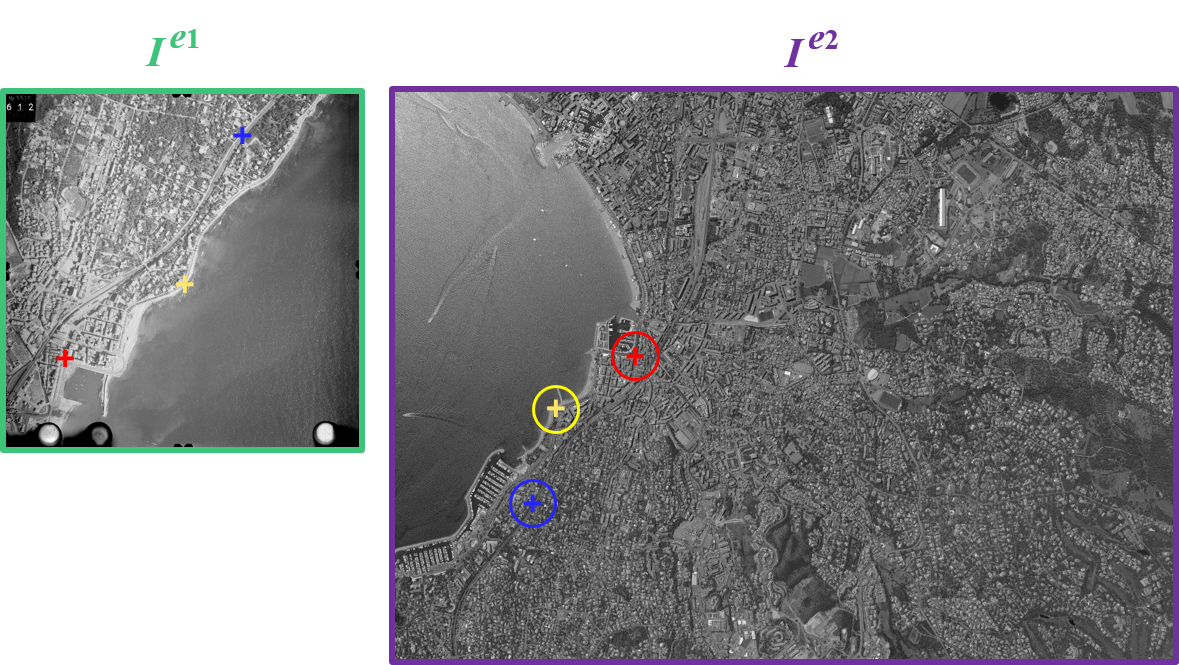
\includegraphics[width=1\columnwidth]{images/Chapitre4/guidedexample.png}
		%		\end{minipage}%
		%	}
		\caption{(a) Example demonstration of an image pair, the master image ($I^{e_1}$) and secondary image ($I^{e_2}$) are taken at Fr{\'e}jus in 1954 and 2014 individually. (b) Patch pairs resulted from (a), the original tile zone before buffering is marked as red rectangles.}
		\label{patchexample}
	\end{center}
\end{figure*}

\begin{figure*}[htbp]
	\begin{center}
		\subfigure[Example of keypoint prediction]{
			\begin{minipage}[t]{1\linewidth}
				\centering
				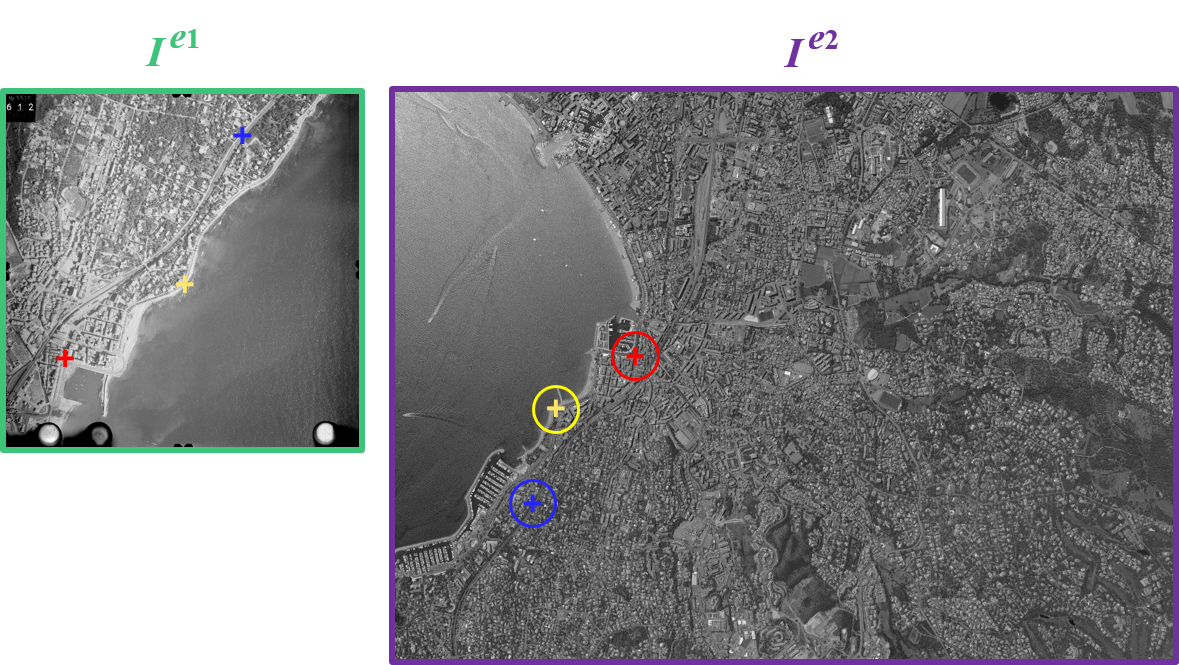
\includegraphics[width=1\columnwidth]{images/Chapitre4/guidedexample.png}
			\end{minipage}%
		}
		\caption{Example demonstration of keypoint prediction (cross symbols) accompanied with search space (circles) on an image pair, the master image ($I^{e_1}$) and secondary image ($I^{e_2}$) are taken at Fr{\'e}jus in 1954 and 2014 individually.}
		\label{guidedexample}
	\end{center}
\end{figure*}

\subsubsection{Guided matching for hand-crafted features.} 
The patch matching substitute orientated towards hand-crafted features is the guided matching, as shown in Figure~\ref{WorkflowPatch}(d). It leverages the positions of predicted keypoints, {the known scale ratio and rotation differences to narrow down the list of the matching candidates}. In our experiments, we use the SIFT points, but the pipeline is suitable to any hand-crafted extractor.
The strategy {is as follows}:\\
\begin{enumerate}
	\item {Compute the scale ratio $R_{scl}$ and the rotation $D_{rot}$ between two images by sequentially projecting the $I^{e_1}$ image corners to the co-registered DSM $D_{co}^{e_1}$ and to image $I^{e_2}$;} %\textcolor{red}{Project the image corners of $I^{e_1}$ to the co-registered DSM $D_{co}^{e_1}$, and back-project them to $I^{e_2}$ to estimate the scale ratio $R_{scl}$ and angle difference $D_{ang}$ between images $I^{e_1}$ and $I^{e_2}$.}
	\item Extract keypoints $\mathbf{K}^{e_1}$ in image $I^{e_1}$ and $\mathbf{K}^{e_2}$ in image $I^{e_2}$;
	\item Intersect the keypoints $\mathbf{K}^{e_1}$ with the co-registered DSM $D_{co}^{e_1}$;
	\item Back-project them to image $I^{e_2}$, giving rise to predicted keypoints $\widetilde{\mathbf{K}}^{e_2}$;
	\item Search for a subset of points in $\mathbf{K}^{e_2}$ located within a radius $S$ (100 pixels in our experiments) centered at the predicted positions $\widetilde{\mathbf{K}}^{e_2}$;%\textcolor{green}{(I don't use a distance threshold.)}
	\item {Remove candidate matches whose scales and rotations computed by SIFT are incoherent with $R_{scl}$ and $D_{rot}$ computed from image orientations and the co-registered DSM (i.e., step 1);}
	\item {Find the best match with mutual nearest neighbor and apply the first to second nearest neighbor ratio test~\cite{lowe2004distinctive}.}
\end{enumerate}
For better understanding, in Figure~\ref{guidedexample} we displayed an example of an inter-epoch image pair, with demonstration of keypoint prediction (cross symbols) accompanied with search space (circles) superposed on them.\\

\subsection{Get enhanced matches}
To compute enhanced matches, we apply a 3D-RANSAC filter on the previously obtained tentative matches. {More precisely, we do the following}: (1) for each match $M({\mathbf{K}^{e_1},\mathbf{K}^{e_2}})$, the keypoints $\mathbf{K}^{e_1}$ and $\mathbf{K}^{e_2}$ are projected onto DSM $D_{co}^{e_1}$ and $D_{ini}^{e_2}$ individually to get 3D points $M({\mathbf{G}^{e_1},\mathbf{G}^{e_2}})$; and (2) {the matches} $M({\mathbf{G}^{e_1},\mathbf{G}^{e_2}})$ are iteratively sampled to compute the 3D Helmert transformation RANSAC model:
\begin{equation}
\left [ \begin{array}{c}
{KG}_x^{e_2}\\
{KG}_y^{e_2}\\
{KG}_z^{e_2}
\end{array}
\right ] =\lambda \cdot \mathbf{R} \cdot {\left [ \begin{array}{c}
	{KG}_x^{e_1}\\
	{KG}_y^{e_1}\\
	{KG}_z^{e_1}
	\end{array}
	\right ]} + \left [ \begin{array}{c}
\Delta_x\\
\Delta_y\\
\Delta_z
\end{array}
\right ]. \label{eq:2DSim}
\end{equation}
where $\lambda$ is the scale factor, $\mathbf{R}$ is the rotation matrix and $\left [ \begin{array}{c}
\Delta_x, \Delta_y, \Delta_z
\end{array}
\right ]$ $^{^T}$ is the translation vector.
We set the number of RANSAC iterations to 1000, and consider matches within $T_r$ of its predicted position as inliers. In our experiment, {$T_r$ was set to 10$\times$$GSD$ where $GSD$ is the mean ground sampling distance in the coordinate frame of epoch ${e_2}$. This distance is computed as the ground distance between two adjacent image pixels.}

\subsection{Get final matches}
In the preceding step we got rid of a substantial number of outliers, however, we believe that not all outliers could be identified. Therefore we apply cross-correlation for final validation. Matches with their correlation scores below a predefined threshold (0.6 in our experiments) are discarded. The correlation window size was set to be large enough to take into account the context around a point (32$\times$32 pixels in our experiment). Figure~\ref{crossc} shows an example of a false match (red) eliminated by cross correlation, while the true match (blue) is kept.
\begin{figure*}[htbp]
	\begin{center}
		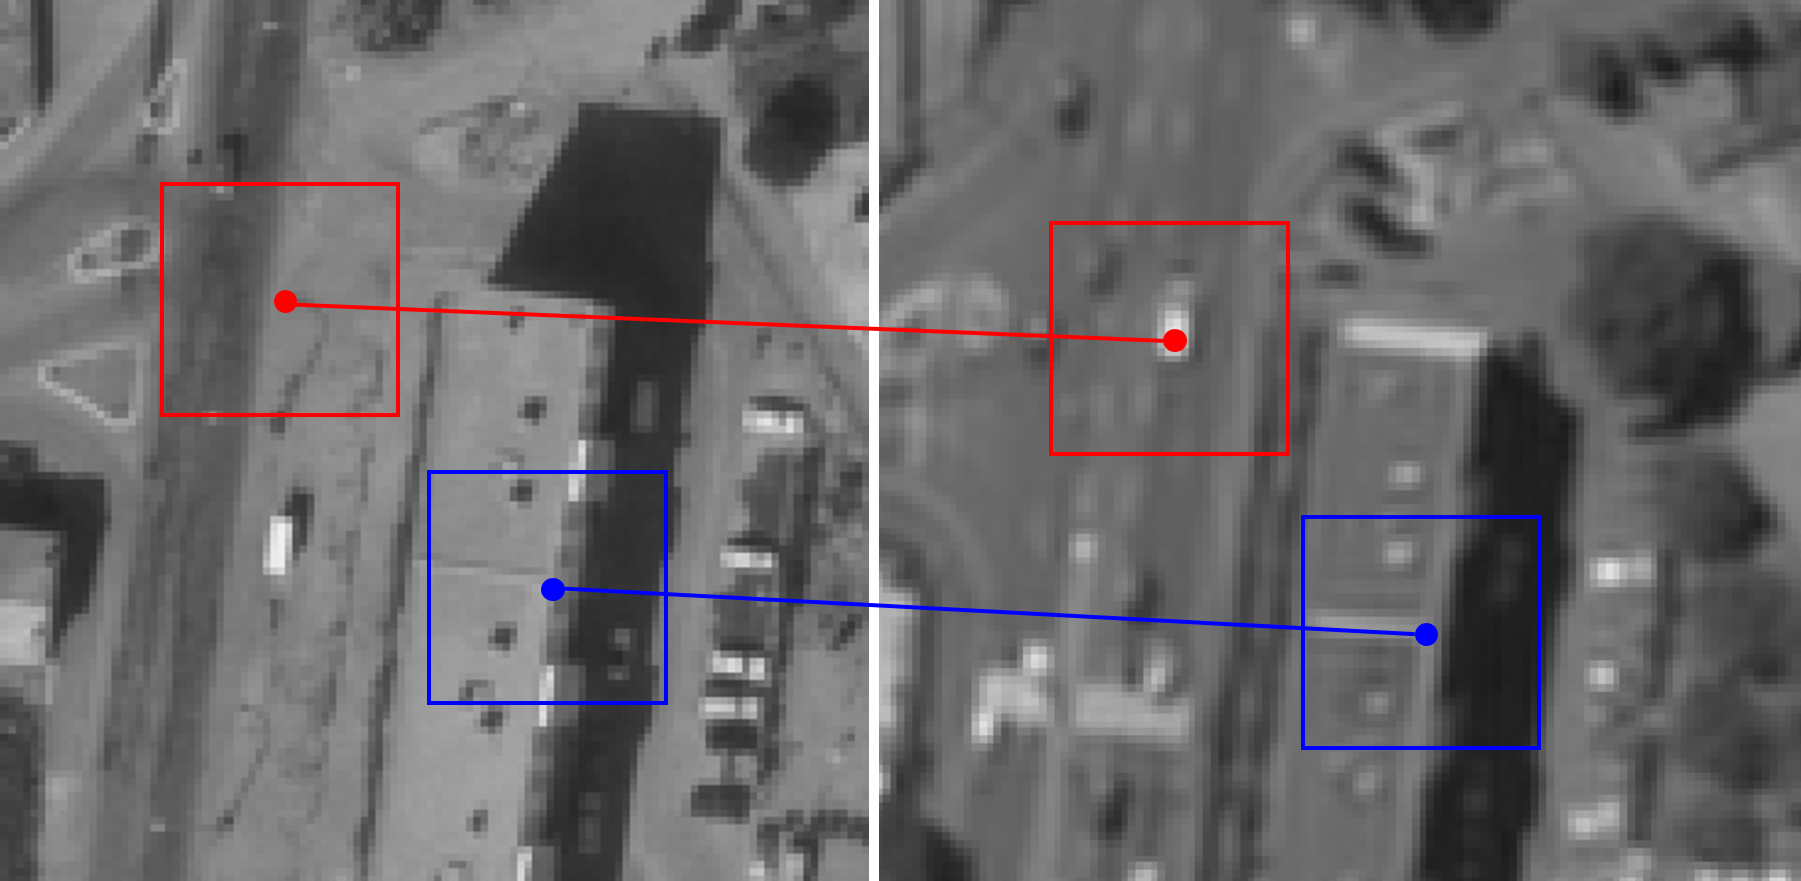
\includegraphics[width=0.8\columnwidth]{images/Chapitre4/tiept.png}
		\caption{Demonstration of the validation with cross-correlation. Considering poor quality of historical images, the window size (blue and red rectangles) was set to 32$\times$32 pixels. False match (red) is eliminated by cross correlation, while true match (blue) is kept.}
		\label{crossc}
	\end{center}
\end{figure*}

\subsection{Combined Processing}
Based on the intra-epoch and inter-epoch feature correspondences, a free network BBA is performed to refine all the image orientations and camera calibrations. If the results need to be analyzed in a metric scale, a spatial similarity transformation will be performed to move the refined acquisitions in an arbitrary reference frame to a metric one. If the precise orientations for one of the epochs were known (i.e., deemed as ground truth), their parameters will be fixed during the BBA and the subsequent spatial similarity transformation will be skipped.
We adopted the Fraser model ~\cite{fraser1997digital} to calibrate the cameras and allowed image-dependent affine parameters, the remaining parameters were
shared among all images.




\section{Experiments}

\section{Conclusion}

\section{Discussion}
